\section{问题四的模型建立与求解}

第四问中，定向源即使距检测点不足1000米，也会因检测点处于发射背面而返回无信号，第三问的单点圆盘排除方法因而失效。我们据此建立``方向覆盖约束下的搜索-清除联合规划模型''，利用多点检测消除方向歧义，将距离与方向联合排查条件纳入第三问的滚动协同框架，安排搜索、定位与清除任务。

\subsection{模型建立}

\subsubsection{定向接收条件}

沿用第三问的状态与行动定义，由于第四问引入了定向干扰源，故我们将单源参数扩展为 \(x=(g,R,\phi,\zeta)\)，其中，\(\phi\) 为发射朝向，\(\zeta=0,1\) 分别表示全向源和定向源。令 \(\boldsymbol d(\phi)=(\cos\phi,\sin\phi)^{\mathsf T}\)，未清除源在检测点 \(s\) 处的接收条件为：
\[
\nu(s;x)=
\begin{cases}
\mathbf 1_{\{\|s-g\|_2\le R\}},&\zeta=0,\\
\mathbf 1_{\{\|s-g\|_2\le R\}}\mathbf 1_{\{\boldsymbol d(\phi)^{\mathsf T}(s-g)\ge0\}},&\zeta=1
\end{cases}
\tag{35}
\]

其中，\(\nu=1\) 表示能够接收信号，内积非负表示检测点位于180°发射半平面内。用式（35）替换第三问反馈更新中的接收条件：有信号时保留 \(\nu=1\) 的参数组合，并加入原有的距离或示向度约束；无信号时保留 \(\nu=0\) 的组合。同一源的位置、半径、朝向和类型保持固定，更新后的组合须满足历次反馈。

清除不受发射朝向限制，第三问的清除反馈更新及式（24）的保证清除区域继续适用。因此，本问新增的约束集中在未知频道的排查过程。

\subsubsection{完整排查与优化目标}

覆盖布局需考虑目标朝向对可观测性的影响\textsuperscript{\cite{ref6}}。单侧检测点可以同时处于发射背面；若检测点从不同方向包围潜在源位置，则至少有一点位于发射正面，如图\ref{fig:old5}所示。结合最小接收半径，这一关系可用于排除区域。

\begin{figure}[H]
\centering
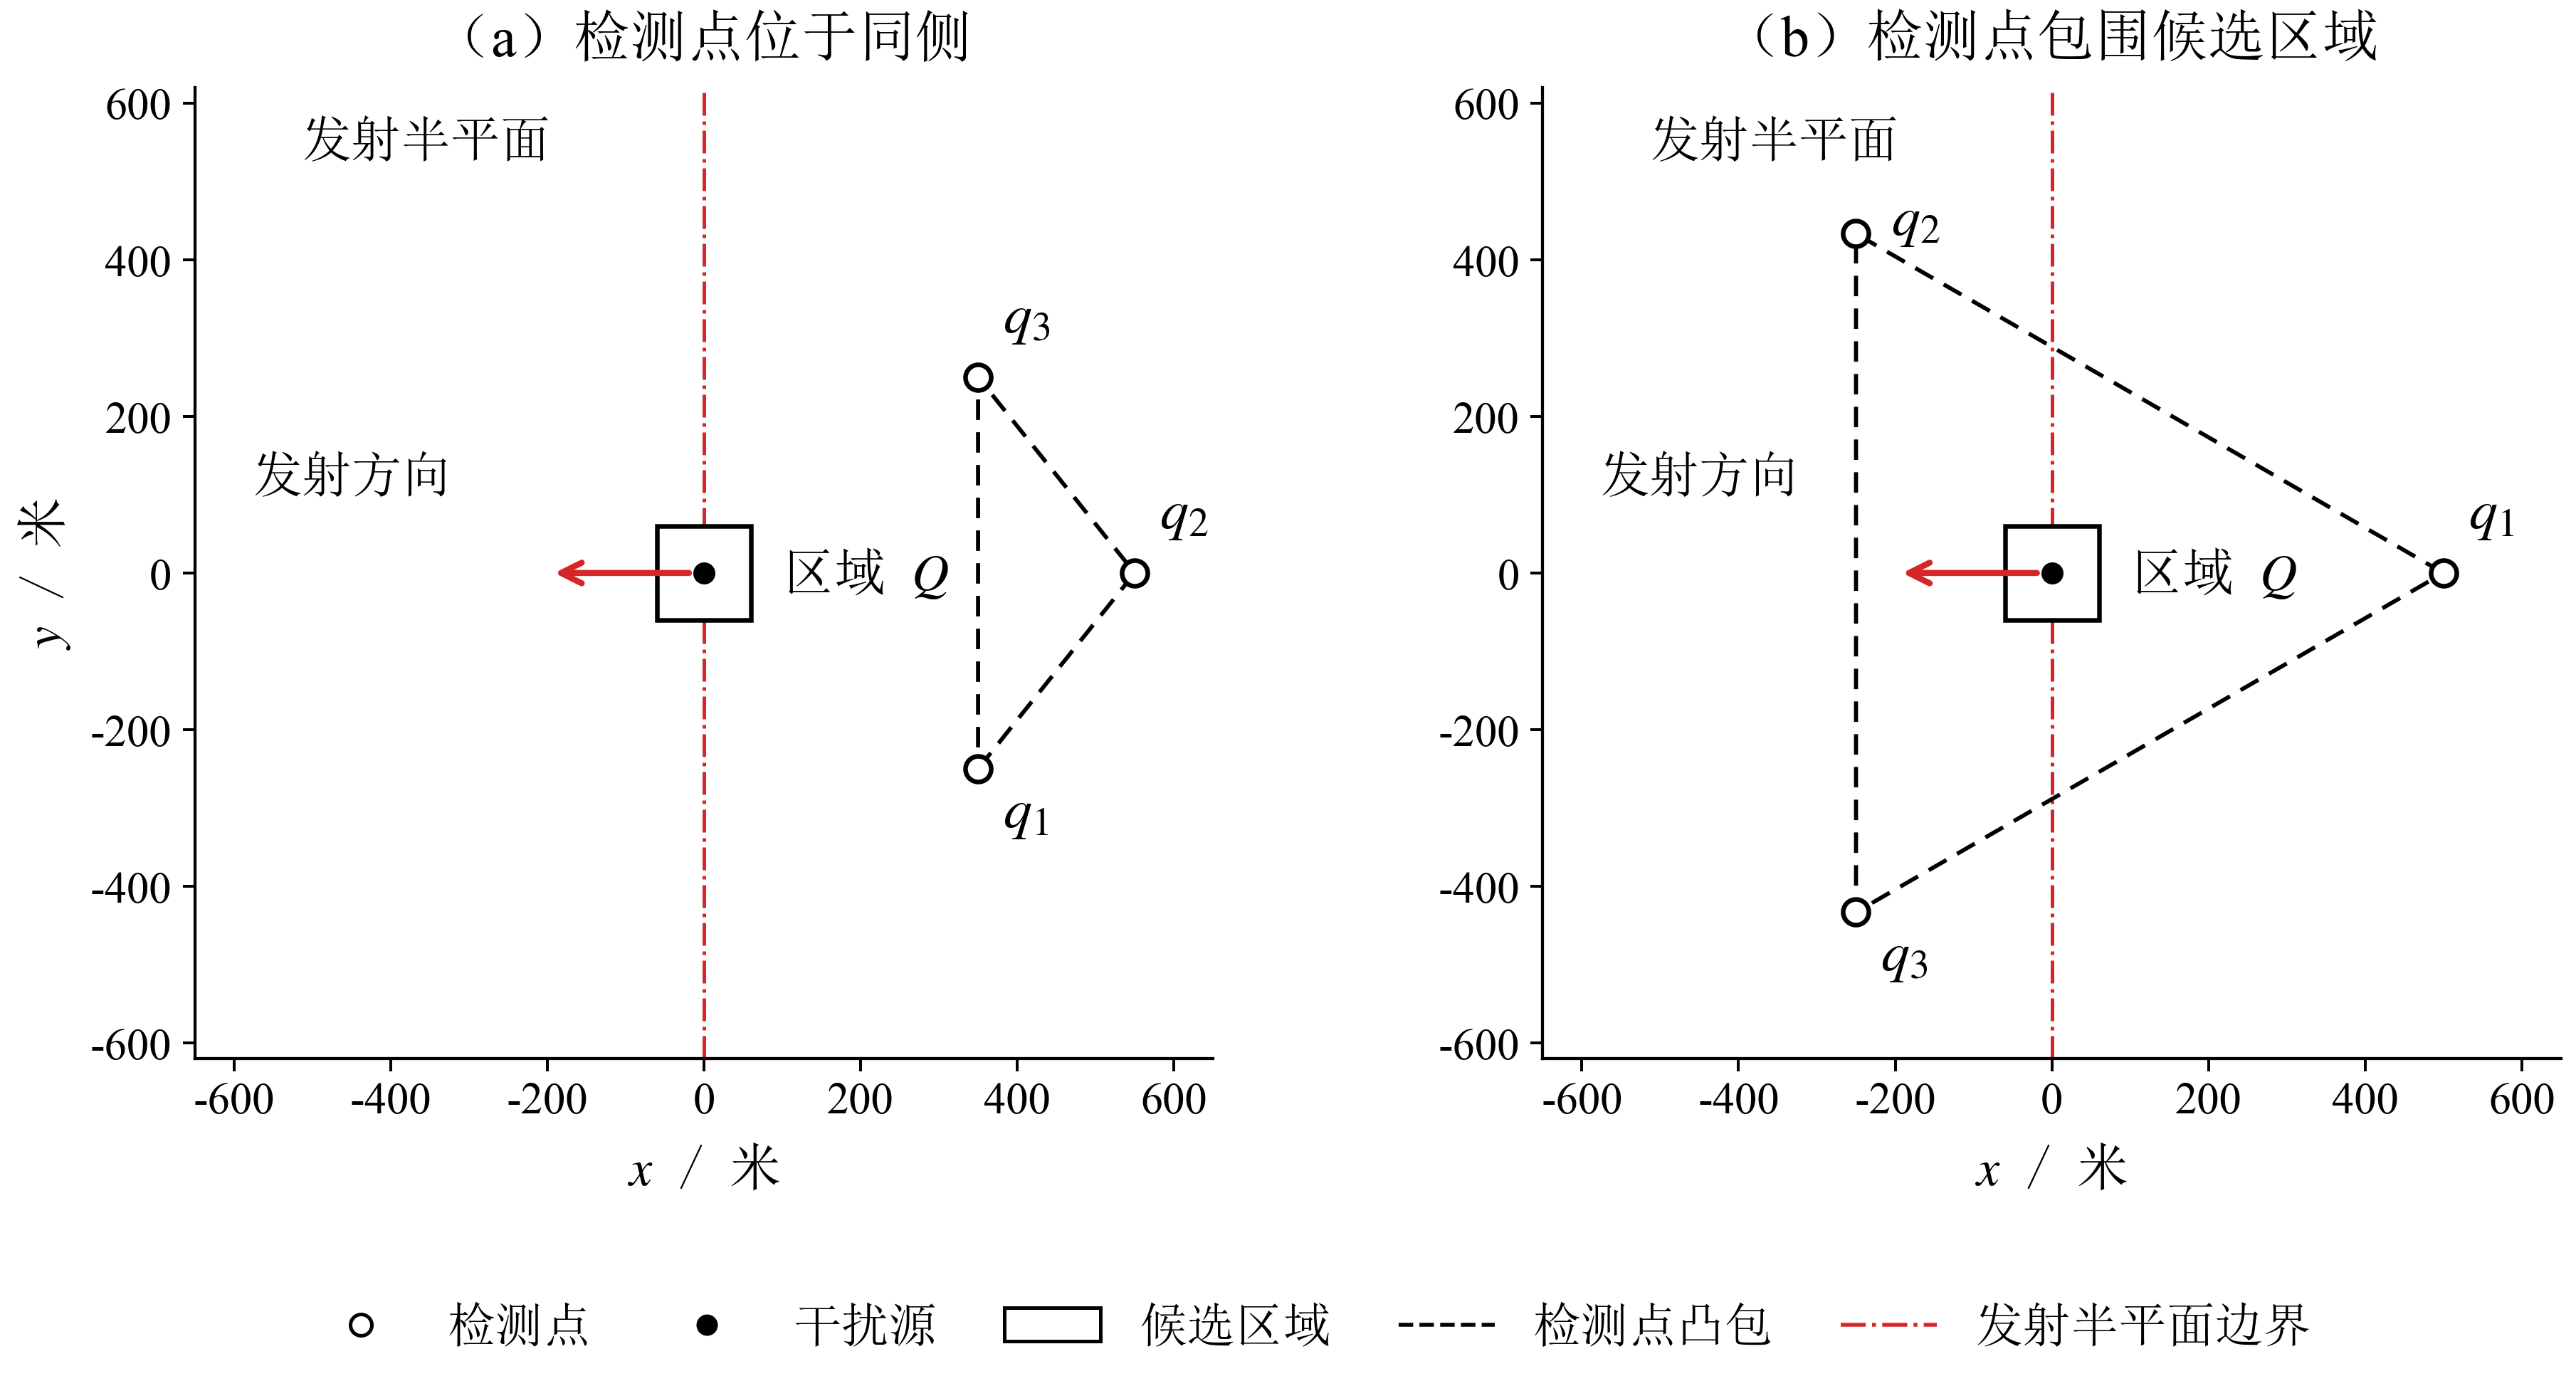
\includegraphics[width=0.96\linewidth,height=0.68\textheight,keepaspectratio]{figures/q4_directional_detection.png}
\caption{单侧检测与包围检测的方向覆盖}\label{fig:old5}
\end{figure}

设 \(Q\) 为候选源区域，\(P_Q\) 为检测点集合。我们要求：
\[
\max_{s\in P_Q}\sup_{g\in Q}\|s-g\|_2<R_{\min},
\qquad Q\subset\operatorname{int}\operatorname{conv}(P_Q),
\qquad R_{\min}=1000\ \text{米}
\tag{36}
\]

第一项保证检测点均在接收半径内，第二项保证检测点包围整个候选区域。式（36）给出与源朝向无关的排除充分条件，具体证明如下。

\begin{propositionbox}
\noindent 命题： 若 \(Q\) 与 \(P_Q\) 满足式（36），且同一频道在各检测点均实际返回无信号，则 \(Q\) 内不存在该频道当前未清除的源。

\noindent 证明： 假设存在源 \(g\in Q\)，全部检测点均在其接收半径内。全向源应被接收，与反馈矛盾；对朝向为 \(\boldsymbol d\) 的定向源，若所有检测点均处于 \(\boldsymbol d^{\mathsf T}(s-g)\le0\) 的半平面，其凸包也在该半平面内，边界上的 \(g\) 不能成为凸包内点，与式（36）矛盾。因此至少一个检测点满足 \(\boldsymbol d^{\mathsf T}(s-g)>0\)，应取得信号，同样与反馈矛盾。得证。
\end{propositionbox}

该条件同时约束后续检测位置。沿用第三问的无信号检测点集合 \(H^-_{c,t}\)、计划检测点集合 \(\mathcal P_{c,t}\) 和未排除区域 \(U_{c,t}\)。对每个潜在位置 \(g\)，从已执行与计划检测点中选出距离足够近的点，要求：
\[
\begin{aligned}
P_{c,t}(g)&=\{s\in H^-_{c,t}\cup\mathcal P_{c,t}:\|s-g\|_2<R_{\min}\},\\
g&\in\operatorname{int}\operatorname{conv}P_{c,t}(g),
\qquad \forall g\in U_{c,t},\ c\in\mathcal N_t
\end{aligned}
\tag{37}
\]

由上述命题可知，若式（37）成立，且相关检测均已完成并返回无信号，则 \(U_{c,t}\) 中不存在频道 \(c\) 未清除的源，可据此完成剩余排查。

终止条件沿用式（27）：已发现源全部清除，且未知频道的候选区域全部排空。

完整排查条件确定了怎样结束任务，路线选择则决定取得这些检测结果所需的时间。我们以式（37）替换第三问式（26）的圆盘覆盖约束，沿用式（28）---（30）的行动代价、完整退出时间及其期望最小化目标。累计时间包括最后一次清除后继续排查的耗时。

\subsection{模型的滚动求解}

\subsubsection{检测点生成与任务安排}

我们将剩余区域划分为可细分的凸多边形，逐块检验式（36）。对每块选定同一组检测点，检查全部顶点到这些点的距离及顶点是否位于其凸包内部。由凸性，顶点满足条件可保证整块区域满足条件；未通过检验的部分继续细分或保留。

初始巡测后，从满足式（37）的候选布局中选择计划检测点。执行巡测任务前，尝试将检测点移向现有路线或附近目标，仅接受保持式（37）且缩短路程的调整；删除检测点也须保持该条件。这样，已发现目标能够影响后续站位，剩余区域仍保留完整的检测安排。

巡测与已发现源的定位清除共同进入路线。巡测任务以检测点为代表位置，目标任务以当前定位区域的最小包围圆圆心为代表位置；定位区域较大且后续巡测可补充观测的目标暂缓访问，仍保留在待清除集合中。访问目标时继续测向或尝试清除，清除失败则根据反馈更新位置范围。

\subsubsection{后续检测与路线代价估计}

不同访问次序会改变新源被发现的时刻，进而改变后续检测次数和定位绕行。为估计这部分代价，我们选取有限的参数组合 \(x=(g,R,\phi,\zeta)\)，组成 \(\widehat{\mathcal H}_t\)。每完成一站对未知频道的巡测，删除在该站本应可见的组合；剩余组合用于预测未知源在后续检测点的可见性。

记已发现源数为 \(k_t\)，组合保留比例为 \(r_t=|\widehat{\mathcal H}_t|/|\widehat{\mathcal H}_0|\)。以 \(r_t\) 近似单源尚未被发现的概率，在总源数10至16的范围内采用权重 \(w_n=\binom n{k_t}r_t^{n-k_t}\)，估计剩余源数及各巡测站的检测频道数：
\[
\begin{aligned}
\widehat M_t&=
\frac{\displaystyle\sum_{n=\max(10,k_t)}^{16}(n-k_t)w_n}
{\displaystyle\sum_{n=\max(10,k_t)}^{16}w_n},\\
\widehat u_j&=u_t-\widehat M_t\left(1-\frac{|\widehat{\mathcal H}_{j^-}|}{|\widehat{\mathcal H}_t|}\right)
\end{aligned}
\tag{38}
\]

其中，\(u_t\) 为当前未知频道数，\(\widehat{\mathcal H}_{j^-}\) 为路线到达第 \(j\) 个巡测站前尚未覆盖的组合，\(\widehat M_t\) 和 \(\widehat u_j\) 分别为预计剩余源数与该站预计检测频道数。组合为空时取 \(\widehat M_t=0\)、\(\widehat u_j=u_t\)；已发现16个源时取 \(\widehat M_t=0\)。这些数值仅参与路线比较，排查完成仍依据真实反馈判断。

设 \(\sigma\) 为从当前位置出发的任务路线，\(L_t(\sigma)\) 为依次访问任务代表位置的路程，\(\mathcal S(\sigma)\) 为其中的巡测任务，\(\eta\) 为途中补测方案。为比较各路线完成巡测和定位的代价，将移动、检测与定位绕行换算为秒，并计入补测的预计作用：
\[
\widehat T_t(\sigma,\eta)=\frac{L_t(\sigma)}5
+6\sum_{j\in\mathcal S(\sigma)}\widehat u_j
+\frac{\widehat L_{\mathrm{refine},t}(\sigma)}5
-\frac{B_t(\sigma,\eta)}{10}
\tag{39}
\]

其中，\(\widehat L_{\mathrm{refine},t}\) 根据沿途新可见的组合估计定位细化的附加路程。\(B_t\) 用于比较途中补测的定位改进与检测开销：每个目标的预计定位半径收缩上限取300米，扣除30米检测等效路程后求和。移动按5米/秒换算，巡测按检测与切频合计6秒/频道估计；补测改进乘权重 \(1/2\) 后换算为时间，得到 \(B_t/10\)。实际行动耗时仍按式（28）累计。

\subsubsection{路线选择}

我们采用迭代局部搜索启发式算法调整任务次序，并构造以不同巡测站为首任务的替代路线。对生成的有限路线与补测方案集合 \(\Sigma_t\)，选择：
\[
(\sigma_t^*,\eta_t^*)\in\arg\min_{(\sigma,\eta)\in\Sigma_t}\widehat T_t(\sigma,\eta)
\tag{40}
\]

\subsubsection{滚动求解步骤}

\textbf{Step 1　初始化并巡测。} 按第三问初始化位置与频道状态，设置候选参数组合，完成初始巡测，取得各频道的首批反馈。

\textbf{Step 2　生成当前任务。} 按8.2.1节生成满足式（37）的计划检测点，与已发现源的定位清除任务共同组成当前任务集合。

\textbf{Step 3　选择任务路线。} 利用迭代局部搜索及不同首站构造候选路线，按式（38）估计检测频道数、式（39）计算路线代价，由式（40）选出当前路线。

\textbf{Step 4　执行首项任务。} 巡测任务在保持式（37）的条件下调整检测点，并执行途中补测与站点检测；目标任务执行定位与清除。途中补测获得有效新信息时，转入Step 5。

\textbf{Step 5　更新检测信息。} 按8.1.1节更新已发现源的定位范围与频道状态，利用实际无信号记录及式（36）更新未排除区域；一站未知频道巡测完成后，删除在该站本应可见的候选参数组合。

\textbf{Step 6　判断是否结束。} 满足式（27）时退出，并按式（29）记录完整耗时；否则返回Step 2。已发现源清除完毕而未知频道仍有未排除区域时，继续巡测。

\subsection{实验验证}

参数确定后，我们使用500个新随机种子检验完整退出情况与耗时。场景按演练分布生成，测向误差采用按频道区分的固定平滑空间场。源真值仅供运行结束后的评价；每源耗时先以各例完整退出时间除以该例原始源数，再跨例统计。结果见表\ref{tab:old8}。

\begingroup
\small
\setlength{\tabcolsep}{4pt}
\setlength{\TableInnerWidth}{\dimexpr\linewidth-2\tabcolsep\relax}
\renewcommand{\arraystretch}{1.22}
\begin{longtable}{@{}>{\centering\arraybackslash}p{0.700\TableInnerWidth}>{\centering\arraybackslash}p{0.300\TableInnerWidth}@{}}
\caption{独立500例的运行结果}\label{tab:old8}\\
\toprule
指标 & 结果 \\
\midrule
\endfirsthead
\multicolumn{2}{c}{表\thetable\quad 独立500例的运行结果（续）}\\
\toprule
指标 & 结果 \\
\midrule
\endhead
\midrule
\multicolumn{2}{r}{续下页}\\
\endfoot
\bottomrule
\endlastfoot
全清且正常退出案例数 & 500 \\
剩余源总数 & 0 \\
平均完整退出时间 / 秒 & 5282.57 \\
平均每源耗时 /（秒/源） & 416.13 \\
每源耗时95\%分位数 /（秒/源） & 556.07 \\
\end{longtable}
\endgroup

500例均完成全部清除并正常退出，统计时间包含失败清除与末段排查。图\ref{fig:old6}显示，每源耗时中位数为405.21秒/源，中间50\%的案例位于356.73至480.41秒/源。按相同口径统计，移动耗时为306.20秒/源，占总耗时约73.6\%，是本组测试的主要时间开销。

\begin{figure}[H]
\centering
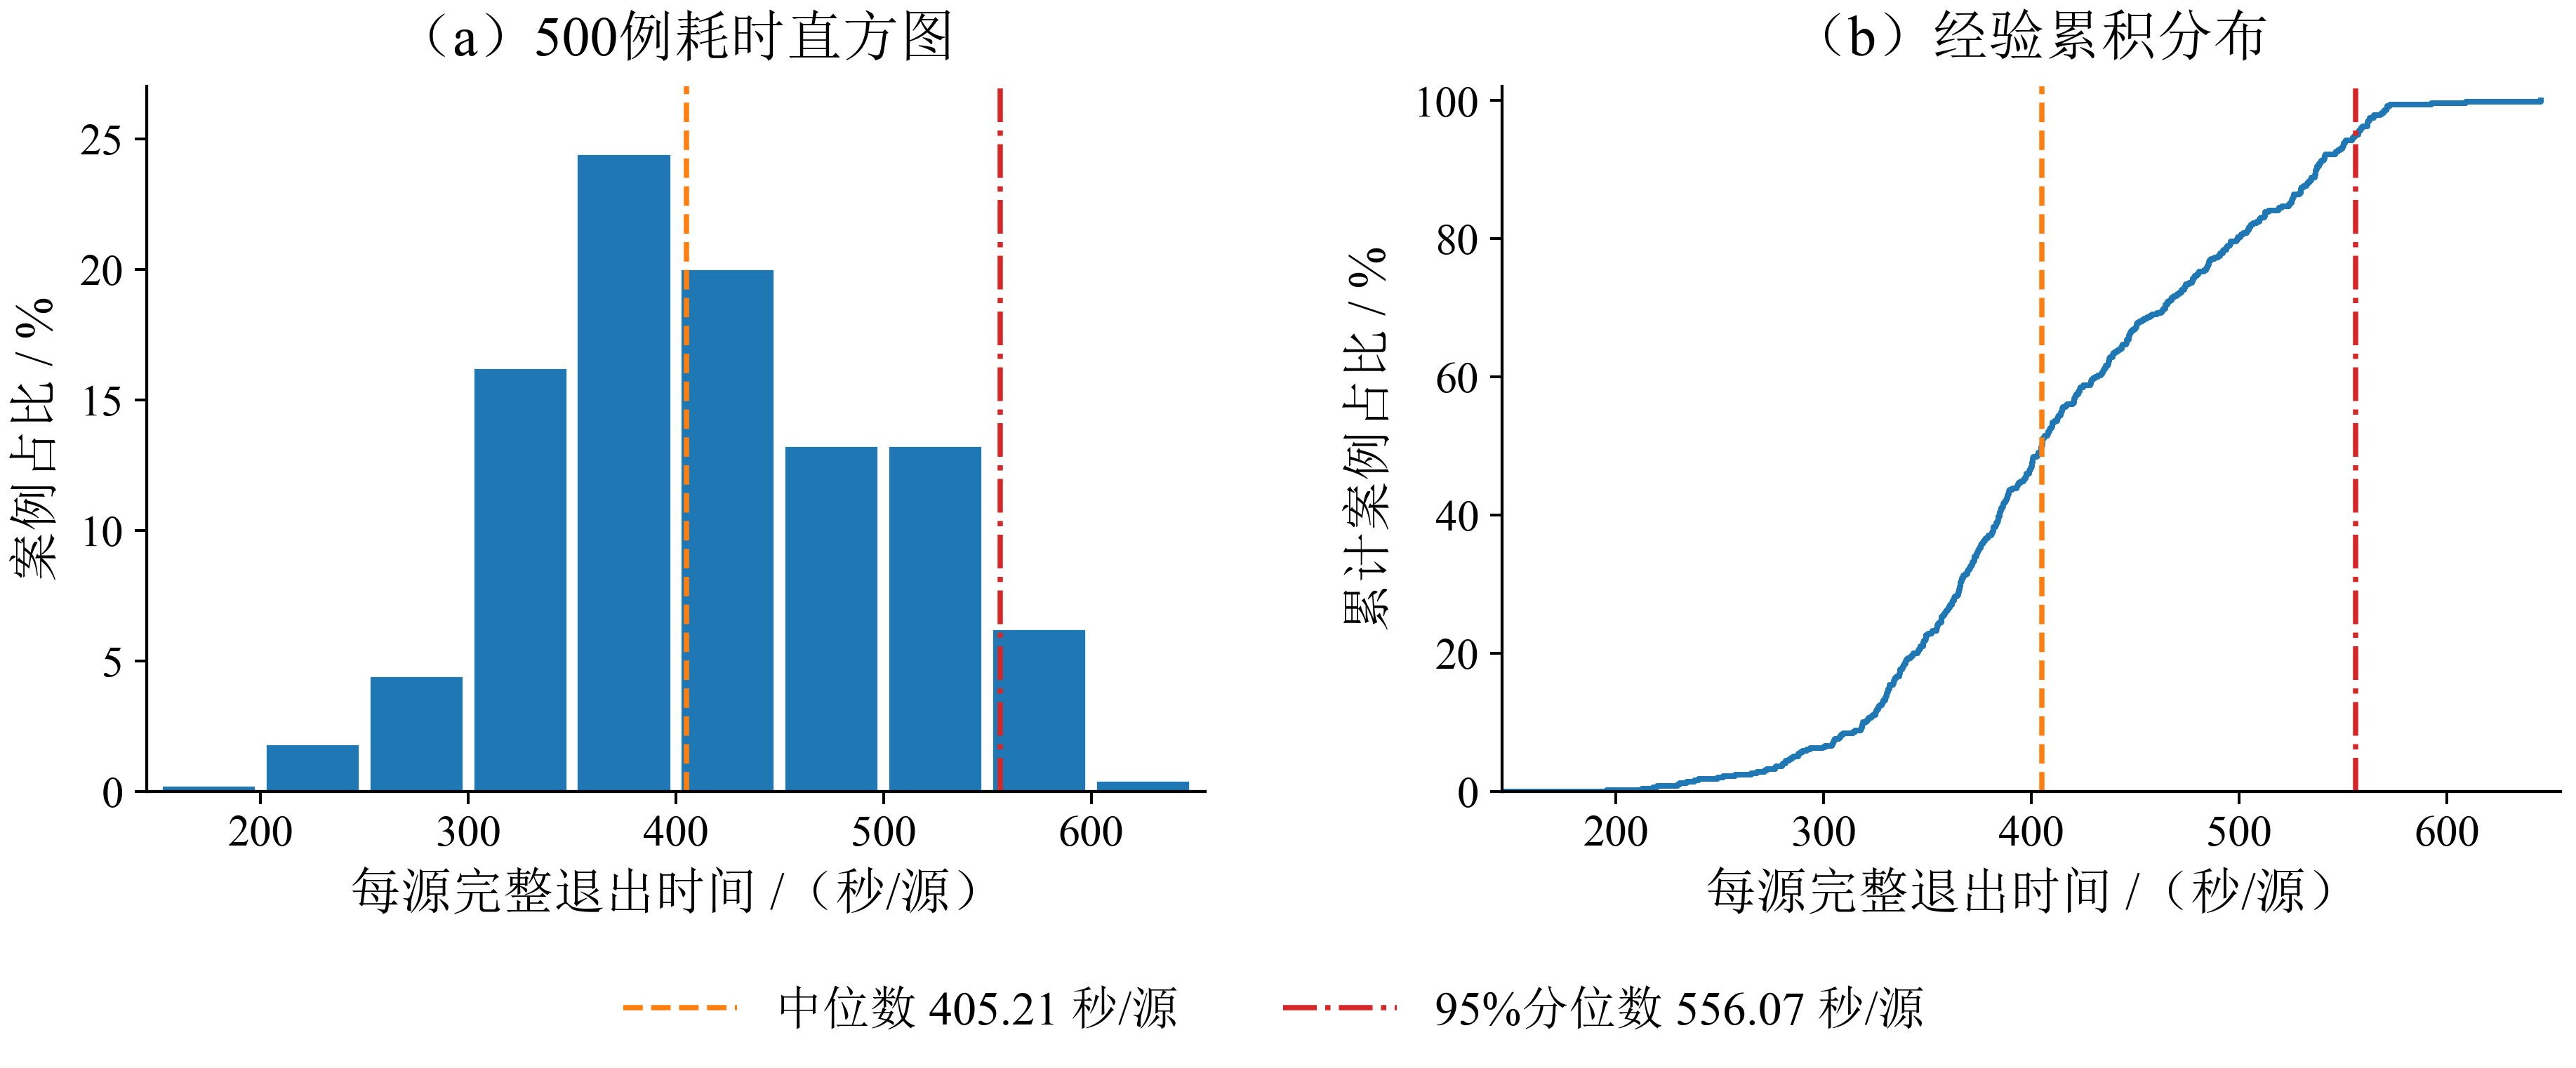
\includegraphics[width=0.96\linewidth,height=0.68\textheight,keepaspectratio]{figures/q4_time_distribution500.png}
\caption{第四问每源完整退出耗时的经验分布}\label{fig:old6}
\end{figure}

图\ref{fig:q4-example-traces}展示此前200例验证中两个案例的完整轨迹。灰线表示巡测与清除，蓝线表示最后清除后的排查，蓝色方形标示退出位置。两例均清除了全部13个源，末段排查分别耗时115.10秒和86.48秒。源位置采用运行结束后的真值。

\begin{figure}[H]
\centering
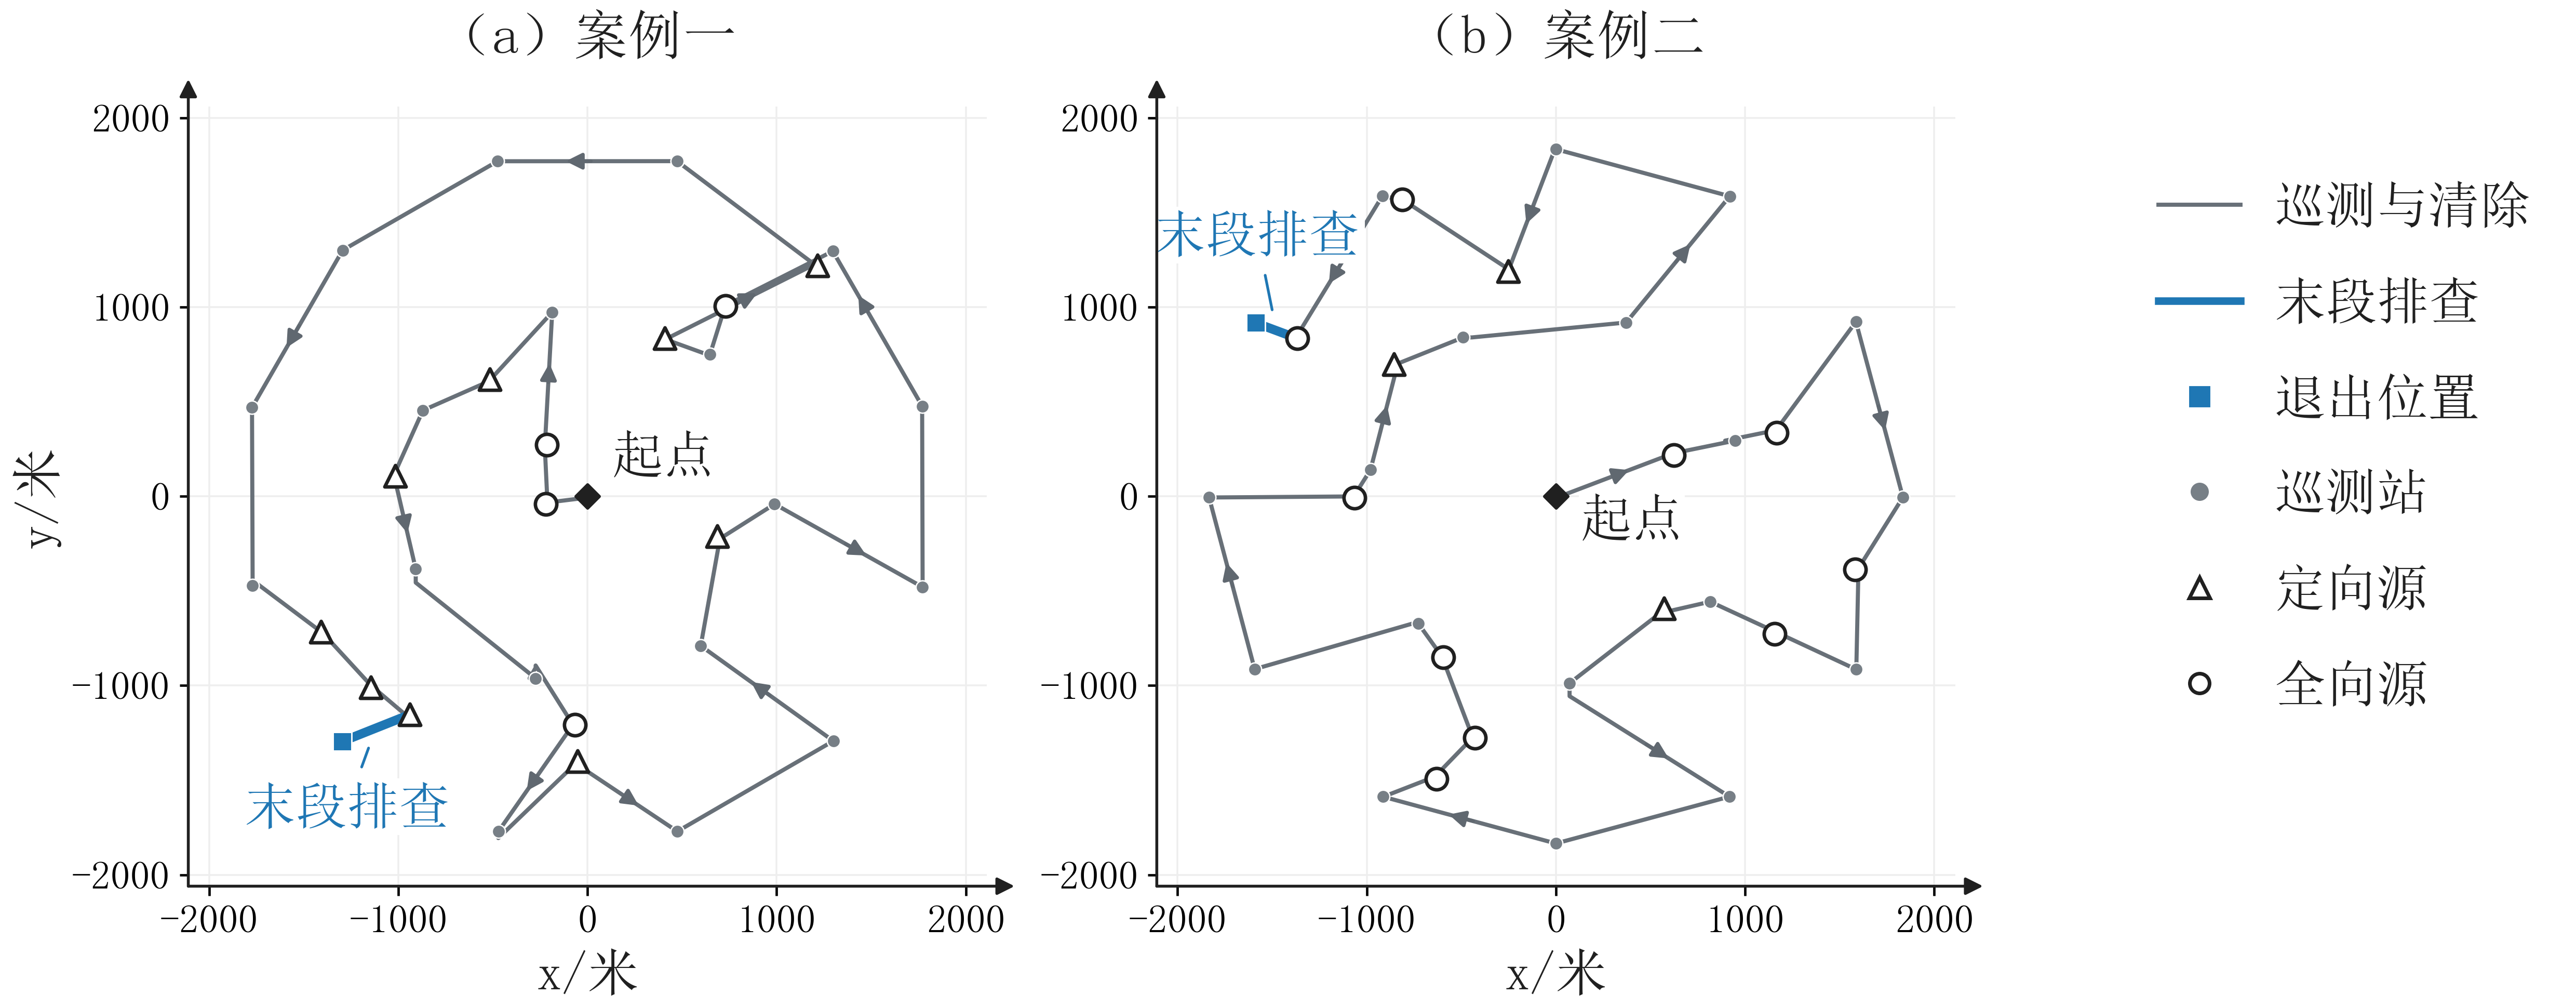
\includegraphics[width=0.99\linewidth,keepaspectratio]{figures/q4_example_trace_cases.png}
\caption{两个案例的完整行动轨迹}\label{fig:q4-example-traces}
\end{figure}

\Needspace{12\baselineskip}
\subsection{正式测试结果}

第四问的三次正式测试均清除了全部干扰源，结果见表\ref{tab:old9}，两项时间分别按第三问正式测试中的虚拟任务耗时与现实执行时长统计。

\begin{table}[H]
\centering
\small
\setlength{\tabcolsep}{4pt}
\setlength{\TableInnerWidth}{\dimexpr\linewidth-6\tabcolsep\relax}
\renewcommand{\arraystretch}{1.22}
\caption{问题4正式测试结果}\label{tab:old9}
\begin{tabular}{@{}>{\centering\arraybackslash}p{0.390\TableInnerWidth}>{\centering\arraybackslash}p{0.170\TableInnerWidth}>{\centering\arraybackslash}p{0.260\TableInnerWidth}>{\centering\arraybackslash}p{0.180\TableInnerWidth}@{}}
\toprule
测试案例编码 & 清除干扰源个数 & 平均定位清除时间 /（秒/源） & 程序运行时间 / 秒 \\
\midrule
XH33-K2C8-8MEP-YJYN & 15 & 335.286 & 6.373 \\
2VV2-BRDE-U2HD-F5PU & 11 & 498.589 & 6.543 \\
CPE4-6NCH-EFMC-8RVG & 10 & 542.428 & 5.932 \\
\bottomrule
\end{tabular}
\end{table}

\subsection{灵敏度分析与消融实验}

开发集与独立验证集各取100个随机种子，各设置按同种子配对。独立验证中，四种设置均完成全部清除并正常退出，结果见表\ref{tab:q4-sensitivity-ablation}。

\begingroup
\small
\setlength{\tabcolsep}{4pt}
\setlength{\TableInnerWidth}{\dimexpr\linewidth-4\tabcolsep\relax}
\renewcommand{\arraystretch}{1.12}
\begin{longtable}{@{}>{\centering\arraybackslash}p{0.450\TableInnerWidth}>{\centering\arraybackslash}p{0.330\TableInnerWidth}>{\centering\arraybackslash}p{0.220\TableInnerWidth}@{}}
\caption{补测权重与途中补测机制的独立验证结果}\label{tab:q4-sensitivity-ablation}\\
\toprule
实验设置 & 平均每源耗时 /（秒/源） & 相对基准变化 \\
\midrule
\endfirsthead
\multicolumn{3}{c}{表\thetable\quad 补测权重与途中补测机制的独立验证结果（续）}\\
\toprule
实验设置 & 平均每源耗时 /（秒/源） & 相对基准变化 \\
\midrule
\endhead
\midrule
\multicolumn{3}{r}{续下页}\\
\endfoot
\bottomrule
\endlastfoot
补测收益权重0.25 & 420.82 & -0.02\% \\
补测收益权重0.50（基准） & 420.89 & 0.00\% \\
补测收益权重1.00 & 420.08 & -0.19\% \\
关闭途中补测及奖励 & 425.62 & +1.12\% \\
\end{longtable}
\endgroup

（1）灵敏度分析。 将式（39）中的补测收益权重取0.25、0.50和1.00，平均每源耗时极差为0.81秒，仅占基准的0.19\%。两种权重变体分别有98例和96例与基准轨迹相同，权重调整对行动次序影响较小。

（2）消融实验。 关闭途中补测及其奖励后，平均每源耗时增加4.73秒，配对差的95\%自助置信区间为[2.24，7.55]秒。其中，移动耗时增加4.62秒/源，是新增代价的主要来源，表明途中补测减少了后续定位绕行。
